\pdfoptionpdfminorversion=5
\documentclass{beamer}

\mode<presentation>
{
  \usetheme{Malmoe}
}

\usepackage{listings}
\usepackage[english]{babel}
\usepackage[latin1]{inputenc}
\usepackage{times}
\usepackage[T1]{fontenc}
\usepackage{eurosym}

\title[CF3 demo]{Coolfluid 3: Demonstration of current capabilities}

\date{16 Nov 2011}

\begin{document}

\section{Introduction}

\begin{frame}
 \frametitle{Coolfluid 3}
\begin{columns}
\begin{column}{5cm}
\begin{itemize}
 \item Started based on CF2 experience, as natural evolution
 \item Focus on flexibility and inter-operability between solvers
 \item Inter-institutional project
 \begin{itemize}
  \item IDIHOM
  \item PhD projects
  \item Institutions involved: VKI, VUB, RMA
 \end{itemize}
\item Open source
\end{itemize}
\end{column}
\begin{column}{5cm}
\begin{center}
 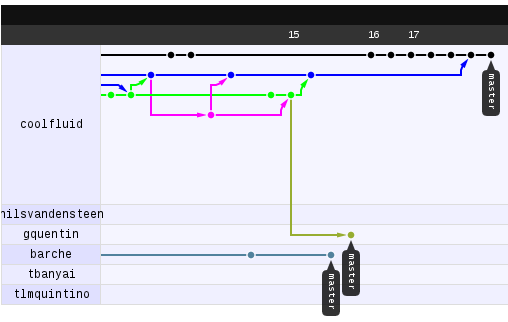
\includegraphics[width=5cm]{figs/github}\\
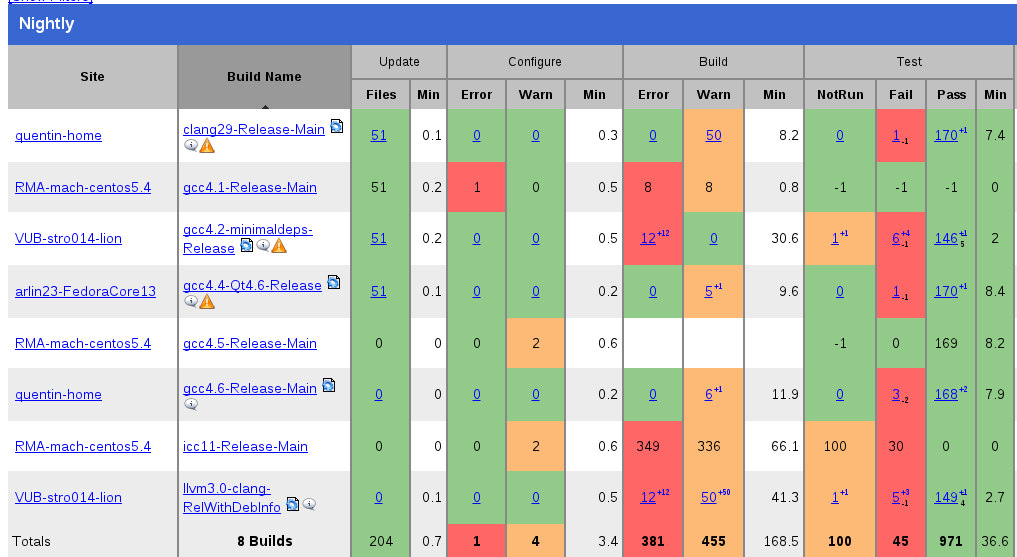
\includegraphics[width=5cm]{figs/dash}
\end{center}
\end{column}
\end{columns}
\end{frame}

\section{Component System}

\begin{frame}
 \frametitle{Component System}
\begin{itemize}
 \item Structure
 \begin{itemize}
  \item Tree of components, parents own children
  \item Access through ``file system'' path interface
 \end{itemize}
 \item Dynamic API
 \begin{itemize}
  \item Configuration using options
  \item Function calls through ``signals''
  \item Network-transparent
  \item Used for automatic UI and script binding interface
 \end{itemize}
 \item C++ API in the ``common'' library
\end{itemize}
\end{frame}

\section{GUI}

\begin{frame}
 \frametitle{GUI}
 \begin{itemize}
  \item Client-server system
  \item Server can control a parallel simulation on a cluster
  \item Mesh visualization using Paraview
  \item Dynamic generation, plugin authors don't need to do GUI programming
 \end{itemize}
\end{frame}

\section{Mesh}

\begin{frame}
  \frametitle{Mesh}
    \begin{block}{Component environment:}
    \begin{itemize}
      \item Multiple meshes
      \item Nesting of regions (CAD)
    \end{itemize}
    \end{block}
    \begin{block}{Features:}
    \begin{itemize}
      \item Unstructured
      \item Continuous / Discontinuous fields
      \item High-order
      \item Parallel
    \end{itemize}
  \end{block}
\end{frame}

\frame[containsverbatim]{ \frametitle{CAD-like topology:\; mesh.print\_tree() }
\begin{verbatim}
  Mesh                              Mesh
    + Topology                      Region
        - Flow                      Region
        + AirPlane                  Region
            + Wings                 Region
            |   + LeftWing          Region
            |   |   - Patch1        Region
            |   |   - Patch2        Region
            |   - RightWing         Region
            + Fuselage              Region
                + Quads             Elements
                + Triags            Elements
\end{verbatim}
  % \begin{itemize}
  %   \item Elements are grouped per type inside these regions
  %   \begin{itemize}
  %     \item Memory optimized per element type (connectivity tables)
  %     \item Optimized numerical algorithms per element type possible.
  %   \end{itemize}
  % \end{itemize}
}

\def\colorize<#1>{\temporal<#1>{\color{black!25}}{\color{red!80}}{\color{black}}}

\frame<1>[label=spaces_and_fields]{ \frametitle{Spaces and Fields}
  \begin{block}{Spaces}
    \begin{itemize}
      \colorize<1> \item Parallel representation of the mesh, or part of the mesh
      \colorize<1> \item Continuous/Discontinuous
      \colorize<2> \item Defined by shape-function and connectivity table
      \colorize<3> \item Accurate interpolation between spaces
    \end{itemize}
  \end{block}
{\begin{block}{Fields}
  \begin{itemize}
    \colorize<3> \item Defined in 1 space (Not necessarily the entire mesh)
    \colorize<3> \item Continuous/Discontinuous (e.g. FE / SD)
    \colorize<4> \item Synchronizable using MPI
    \colorize<4> \item Coordinates are a field like any other
  \end{itemize}
\end{block}
}
}


\frame[t]{ \frametitle{Spaces and Fields}
\begin{columns}
\begin{column}{0.6\textwidth}
\begin{center}
  \includegraphics<1>[width=\columnwidth]{figs/spaces_0}
  \includegraphics<2>[width=\columnwidth]{figs/spaces_1}
  \includegraphics<3>[width=\columnwidth]{figs/spaces_2}
  \includegraphics<4>[width=\columnwidth]{figs/spaces_3}
\end{center}                                   
\end{column}
\begin{column}[b]{0.4\textwidth}
  \begin{block}{\color{black} A 2D mesh}
  \begin{itemize}
  \item<2-> \color{red} Geometry space
  \item<3-> \color{blue} Solution space
  \item<4-> \color{brown} Interpolated space
  \end{itemize}
  \end{block}
\end{column}
\end{columns}
}

\againframe<2>{spaces_and_fields}

\frame[containsverbatim]{ \frametitle{Spaces and Fields}
\begin{columns}
\begin{column}{0.45 \textwidth}
\begin{verbatim}
Mesh
+ Topology
| - Flow
|   - Triangles
|   - Quads
+ GeometrySpace
| - Coordinates
| - WallDistance
+ SolutionSpace
  - Coordinates
  - Solution
  - Residual
\end{verbatim}
\end{column}
\begin{column}{0.5 \textwidth}
\begin{verbatim}
Quads
- ElementType
+ Spaces
  + GeometrySpace
  | - ShapeFunction (P1)
  | - ConnectivityTable
  + SolutionSpace
    - ShapeFunction (P3)
    - ConnectivityTable
\end{verbatim}
\end{column}
\end{columns}
}

\againframe<3>{spaces_and_fields}
\againframe<4>{spaces_and_fields}

\frame{ \frametitle{Mesh Manipulations}
\begin{block}{Create new regions and elements}
  \begin{itemize}
    \item Build faces
    \item Remove or merge regions
    \item Reorganize regions
  \end{itemize}
\end{block}
\begin{block}{Create new spaces and fields}
  \begin{itemize}
    \item High-order solution-space
    \item P-multigrid with multiple solution-spaces
    \item Simple to create and access.
  \end{itemize}
\end{block}
}

\frame{ \frametitle{Mesh IO}
\begin{itemize}
  \item[-] Distributed reading\\
  \item[-] Distributed Repartitioning
\end{itemize}
\begin{block}{Generation}
  \begin{itemize}
    \item Line, Rectangle, Box
    \item Scriptable Blocks, with grading
  \end{itemize}
\end{block}
\begin{block}{Input}
  \begin{itemize}
    \item Gmsh, Neutral, CGNS, OpenFOAM dict
  \end{itemize}
\end{block}
\begin{block}{Output}
  \begin{itemize}
    \item Gmsh, Tecplot, VTK (Paraview), Neutral, CGNS
  \end{itemize}
\end{block}
}

\section{Conclusion}

\begin{frame}
 \frametitle{Current abilities}
\begin{itemize}
 \item Python scripting: 
  \begin{itemize}
   \item parametrization
   \item optimalization
   \item error analysis
  \end{itemize}
 \item Spectral difference
 \item Incompressible Finite Element solver
 \item Residual Distribution
 \item Proto language
 \item Parallelization
 \item LSS interface
\end{itemize}

\end{frame}


\end{document}
